\documentclass[3p, authoryear, review]{elsarticle} %review=doublespace preprint=single 5p=2 column
%%% Begin My package additions %%%%%%%%%%%%%%%%%%%
\usepackage[hyphens]{url}

  \journal{Submitted to Journal} % Sets Journal name


\usepackage{lineno} % add
\providecommand{\tightlist}{%
  \setlength{\itemsep}{0pt}\setlength{\parskip}{0pt}}

\usepackage{graphicx}
%%%%%%%%%%%%%%%% end my additions to header

\usepackage[T1]{fontenc}
\usepackage{lmodern}
\usepackage{amssymb,amsmath}
\usepackage{ifxetex,ifluatex}
\usepackage{fixltx2e} % provides \textsubscript
% use upquote if available, for straight quotes in verbatim environments
\IfFileExists{upquote.sty}{\usepackage{upquote}}{}
\ifnum 0\ifxetex 1\fi\ifluatex 1\fi=0 % if pdftex
  \usepackage[utf8]{inputenc}
\else % if luatex or xelatex
  \usepackage{fontspec}
  \ifxetex
    \usepackage{xltxtra,xunicode}
  \fi
  \defaultfontfeatures{Mapping=tex-text,Scale=MatchLowercase}
  \newcommand{\euro}{€}
\fi
% use microtype if available
\IfFileExists{microtype.sty}{\usepackage{microtype}}{}
\usepackage{natbib}
\bibliographystyle{apalike}
\usepackage{longtable,booktabs,array}
\usepackage{calc} % for calculating minipage widths
% Correct order of tables after \paragraph or \subparagraph
\usepackage{etoolbox}
\makeatletter
\patchcmd\longtable{\par}{\if@noskipsec\mbox{}\fi\par}{}{}
\makeatother
% Allow footnotes in longtable head/foot
\IfFileExists{footnotehyper.sty}{\usepackage{footnotehyper}}{\usepackage{footnote}}
\makesavenoteenv{longtable}
\ifxetex
  \usepackage[setpagesize=false, % page size defined by xetex
              unicode=false, % unicode breaks when used with xetex
              xetex]{hyperref}
\else
  \usepackage[unicode=true]{hyperref}
\fi
\hypersetup{breaklinks=true,
            bookmarks=true,
            pdfauthor={},
            pdftitle={USTM Resiliency Sensitivity Analysis},
            colorlinks=false,
            urlcolor=blue,
            linkcolor=magenta,
            pdfborder={0 0 0}}
\urlstyle{same}  % don't use monospace font for urls

\setcounter{secnumdepth}{5}
% Pandoc toggle for numbering sections (defaults to be off)

% Pandoc citation processing

% Pandoc header
\usepackage{booktabs}



\begin{document}
\begin{frontmatter}

  \title{USTM Resiliency Sensitivity Analysis}
    \author[Brigham Young University]{Gregory Macfarlane\corref{1}}
   \ead{gregmacfarlane@byu.edu} 
    \author[Brigham Young University]{Natalie Gray}
   \ead{nat.gray2000@gmail.com} 
      \address[Brigham Young University]{Civil and Environmental Engineering Department, 430 Engineering Building, Provo, Utah 84602}
      \cortext[1]{Corresponding Author}
  
  \begin{abstract}
  The input parameters used in travel demand models contribute to result uncertainty. A coefficient of variation was used to determine the range of possible values for each parameter. Sampling methods can approximate a normal distribution of parameter values with a discrete number of draws. This paper looks at Monte Carlo sampling and Latin Hypercube sampling. A three-step travel demand model is created with a 25-zone dummy model to evaluate if Latin Hypercube sampling reduces the number of draws needed to approximate Monte Carlo sampling. The mean modechoice logsum value was used to evaluate a cumulative standard deviation of values based upon 100 and 600 draws of parameter values for each sampling method. The standard deviation for Latin hypercube samples stabilize between 100 and 200 draws, whereas Monte Carlo samples often haven't stabilized at 600 draws. Latin hypercube sampling does reduce the number of draws needed, to where it can be applied to a large-scale model.
  \end{abstract}
   \begin{keyword} Sensitivity Analysis, Resiliency, Latin Hypercube Sampling\end{keyword}
 \end{frontmatter}

\hypertarget{questions}{%
\section{Questions}\label{questions}}

There exists uncertainty in travel demand models. This is known by transportation planners but the majority do not use any particular method to quantify it. This uncertainty exists to some extent by the variance among input parameters. Two popular sampling methods to draw from the range of possible parameters are Monte Carlo (MC) simulation and Latin Hypercube Sampling (LHS). MC simulation requires large computations to be effective on a statewide model. LHS reduces the number of variants needed, but the amount of reduction is unknown. \citep{yang2013sensitivity}

The research questions are therefore:

\begin{itemize}
\tightlist
\item
  Using a dummy travel demand model, can Latin Hypercube Sampling reduce the iterations needed to approximate random sampling methods (e.g., Monte Carlo simulation)?
\item
  Does this method of sampling have few enough iterations for statewide model application?
\end{itemize}

\hypertarget{methods}{%
\section{Methods}\label{methods}}

To examine the effects of parameter input sensitivity, we developed a trip-based travel model with three steps:

\begin{enumerate}
\def\labelenumi{\arabic{enumi}.}
\tightlist
\item
  trip generation,
\item
  trip distribution, and
\item
  mode choice.
\end{enumerate}

Trip generation, the first step, was conducted using socioeconomic (SE) data from a 25-zone dummy model of the \href{https://github.com/ActivitySim/activitysim}{ActivitySim GitHub repository}. Trip production was estimated using the \href{https://github.com/byu-transpolab/nhts2017}{2017 National Household Travel Survey data} (NHTS2017). The trip productions were summarized by household sizes, vehicles, and workers, and the weighted mean of each trip purpose was taken. The three trip purposes used are Home Based Work (HBW), Home Based Other (HBO), and Non-Home Based (NHB). NHTS2017 data and the SE data were merged based upon their household size, vehicles, and workers with maximum thresholds set as 4 persons, 3 vehicles, and 2 workers per household. Trip attraction was skipped for this analysis.

The second step, trip distribution, used distance and travel time skims from an example in the ActivitySim GitHub repository. The skims were simplified to use auto, nonmotorized, and transit modes. Travel time for auto used the single occupancy vehicle AM time, nonmotorized travel time used the walking distance skim multiplied by a factor of average walking speed, and transit time used the walk to local bus time.

Mode choice, the third step, calculates utilities for the three modes. These utilities were exponentiated, added together, and the natural log was taken to get a logsum value for every origin and destination pair. The utility equations for the mode choice model are as follows:

\begin{equation}
\mathrm{drive\_utility} = (\mathrm{coeff\_ivtt}*\mathrm{auto})+(\mathrm{coeff\_cost}*\mathrm{auto\_cost}*\mathrm{DIST})
\label{eq:driveutil}
\end{equation}
\begin{equation}
\mathrm{nonmo\_utility} = (\mathrm{k\_nmot}+ 20 * (\mathrm{coeff\_walk1}*\mathrm{nonmotor}))
\label{eq:nonmoutil}
\end{equation}
\begin{equation}
\mathrm{trans\_utility} = \mathrm{k\_trn} + (\mathrm{coeff\_ivtt}*\mathrm{transit})
\label{eq:transutil}
\end{equation}

The mode choice parameters (constants and coefficients) were obtained from the \href{https://github.com/byu-transpolab/ustm_resiliency}{USTM Resiliency Model}. These values are shown in Table \ref{tab:MCcoeff} and Table \ref{tab:MCconst}.

\begin{table}

\caption{\label{tab:MCcoeff}Mode Choice Coefficients}
\centering
\begin{tabular}[t]{lrrr}
\toprule
Name & HBW & HBO & NHB\\
\midrule
CIVTT & -0.0450 & -0.0350 & -0.0400\\
CCOST & -0.0016 & -0.0016 & -0.0016\\
CWALK1 & -0.0900 & -0.0700 & -0.0800\\
AUTOCOST & 18.3000 & 18.3000 & 18.3000\\
\bottomrule
\end{tabular}
\end{table}

\begin{table}

\caption{\label{tab:MCconst}Mode Choice Constants}
\centering
\begin{tabular}[t]{lrrr}
\toprule
Name & HBW & HBO & NHB\\
\midrule
K\_TRN & -0.5140 & -0.9853 & -1.3020\\
K\_NMOT & 1.7602 & 0.5448 & -0.5359\\
\bottomrule
\end{tabular}
\end{table}

With this simple three-step model, MC and LHS methods were used to determine the possible combinations of parameter variance. To identify a standard deviation for each parameter, a coefficient of variation was used. A set coefficient of variation of 0.30 was used for all six input parameters \citep{zhao2002propagation}. The standard deviation was equal to 0.30 multiplied by the mean, where the mean values in this situation are the base scenario parameters (as identified in Table \ref{tab:MCcoeff} and Table \ref{tab:MCconst}).

The MC random sampling uses the R function of \texttt{rnorm}. LHS uses the \texttt{lhs} package in R. Since this package only chooses variables on a zero to one scale, the values given use a function to put the random sampling on the right scale needed for the given parameter. The full code for both methods can be found in a public
\href{https://github.com/natmaegray/ustm_resiliency_sensitivity}{GitHub repository}. 100 and 600 draws of random samples for both methods are generated. With these generated parameters, the mode choice model step was run for every set of input parameters for each purpose. The mean logsum value for each run was determined to compare each continuous draw.

\hypertarget{findings}{%
\section{Findings}\label{findings}}

The parameters generated were compared for both sampling methods. Figure \ref{fig:parameter100} shows the distributions for the HBW parameters when using 100 draws, and Figure \ref{fig:parameter600} shows how that changes when using 600 draws. These distributions show that LHS gives normally distributed parameters with fewer draws than MC sampling. At 100 draws LHS shows a nearly perfect normal distribution, where there are some discrepancies for the MC generated parameters. Without looking at the mode choice results, these Figures show that LHS is likely to estimate the full variance of the results with much fewer draws.

\begin{figure}

{\centering 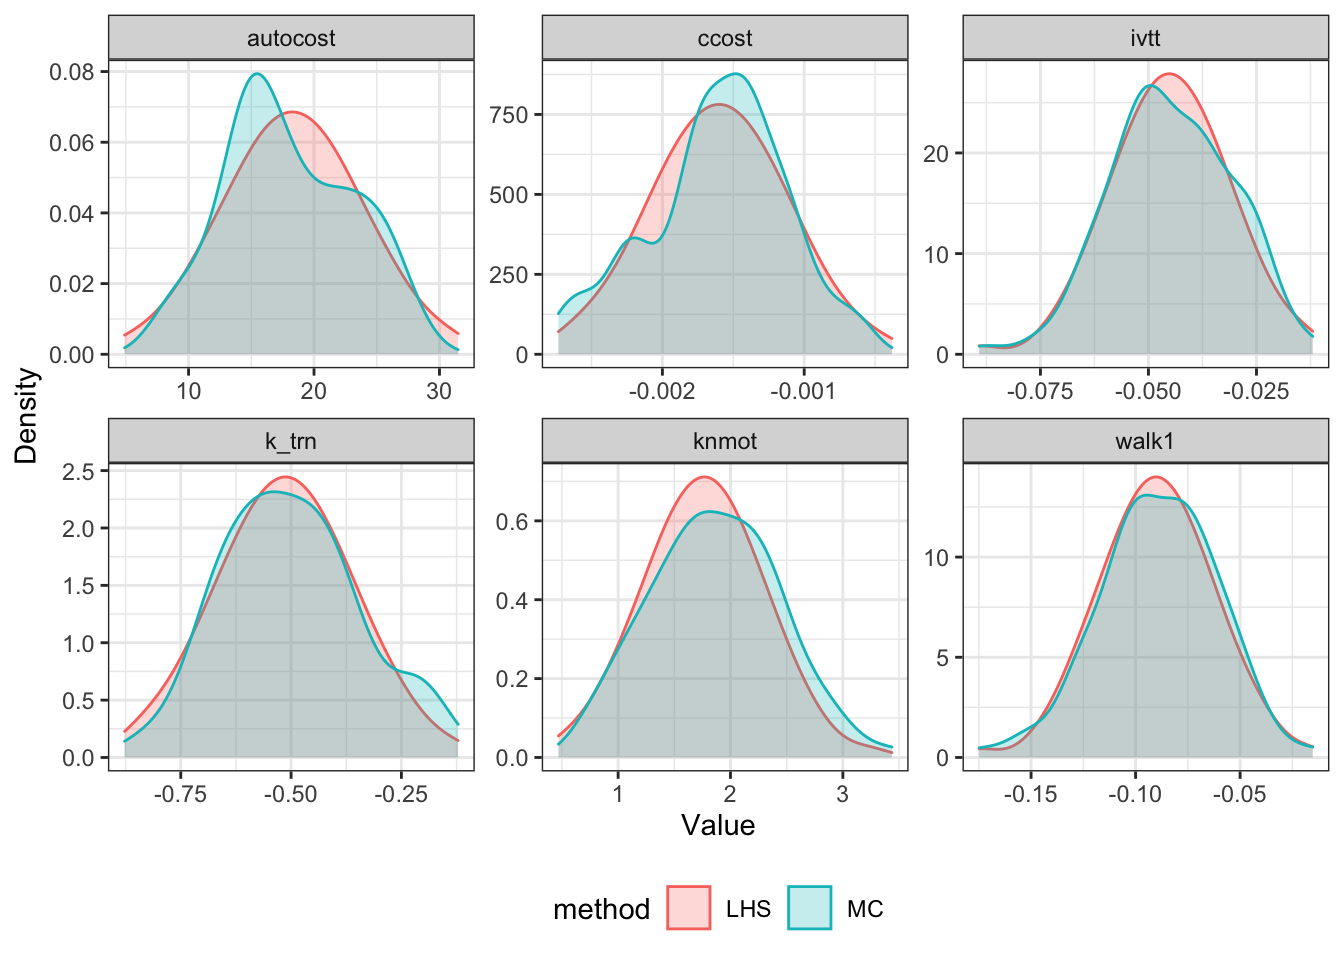
\includegraphics[width=0.75\linewidth]{ustm_resiliency_sensitivity_files/figure-latex/parameter100-1} 

}

\caption{HBW Distributions for Input Parameters with 100 Draws}\label{fig:parameter100}
\end{figure}

\begin{figure}

{\centering 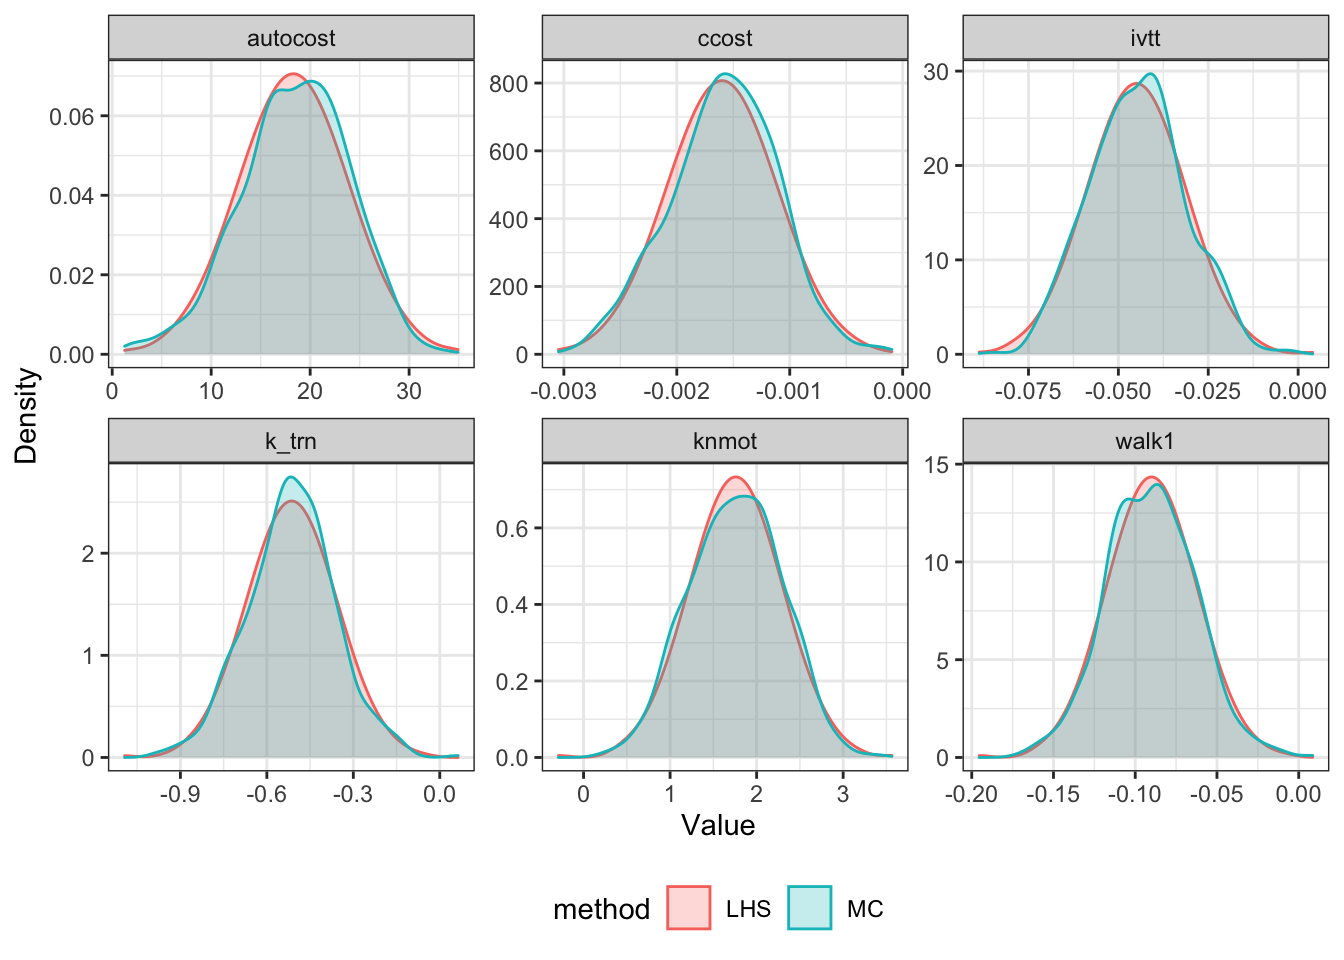
\includegraphics[width=0.75\linewidth]{ustm_resiliency_sensitivity_files/figure-latex/parameter600-1} 

}

\caption{HBW Distributions for Input Parameters with 600 Draws}\label{fig:parameter600}
\end{figure}

To determine if LHS is effective at a reasonable amount of iterations, the standard deviation was calculated for each additional draw. This value shows how much the mean mode choice logsum value for the 25 zones can vary. When the standard deviation for the draws stabilizes, that shows that the amount of generated parameters has captured all of the possible variances of the results. This can be visualized for each purpose. The HBW results for the cumulative standard deviation are shown in \ref{fig:hbwstats}. The results for the other two purposes (HBO and NHB) are in \ref{fig:hbostats} and \ref{fig:nhbstats} respectively.

\begin{figure}

{\centering 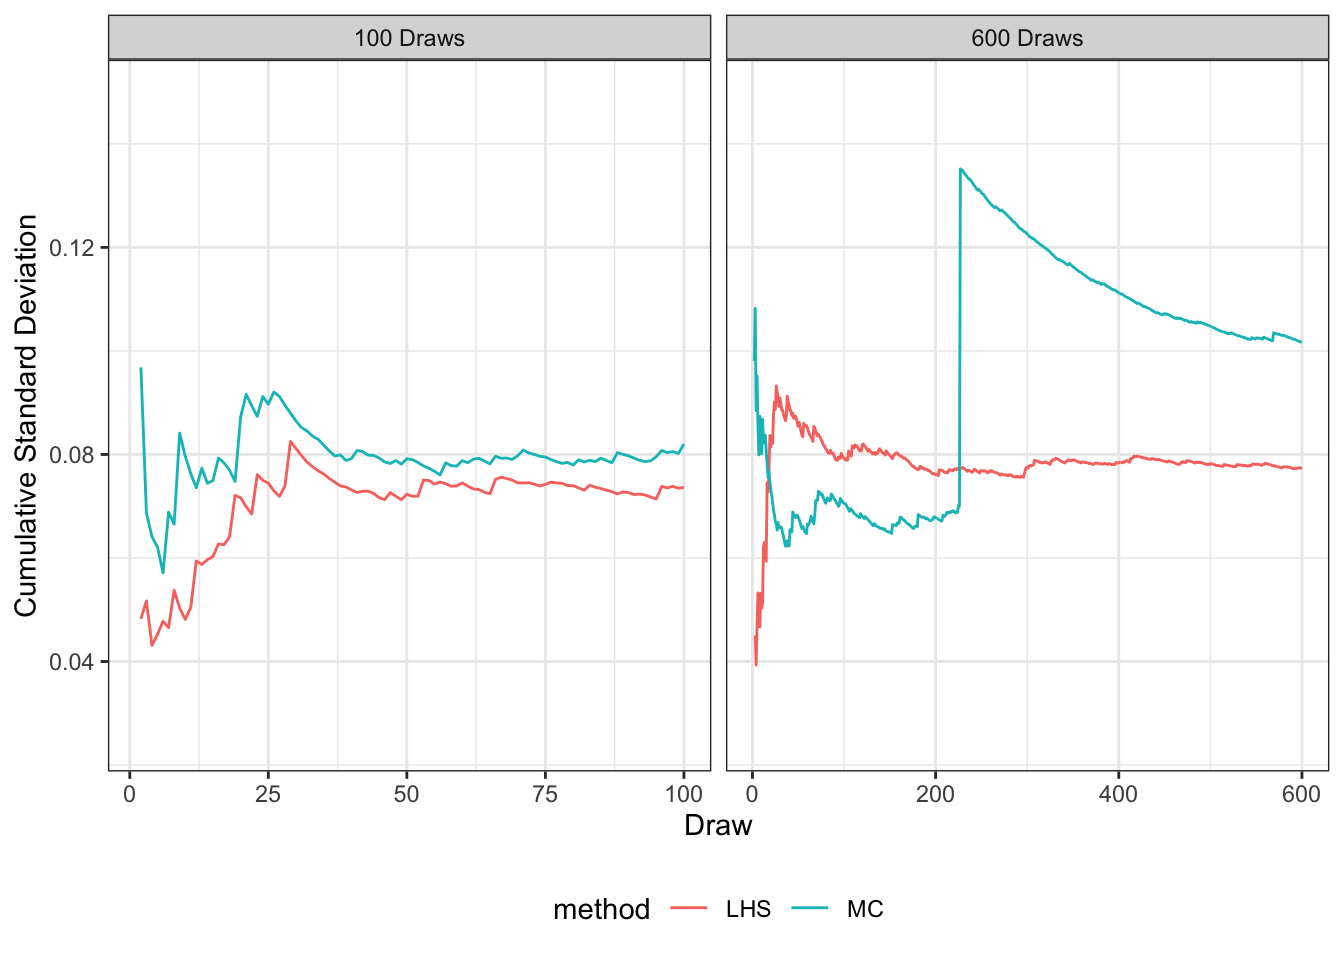
\includegraphics[width=0.75\linewidth]{ustm_resiliency_sensitivity_files/figure-latex/hbwstats-1} 

}

\caption{HBW Mean Logsum Standard Variation with 100 and 600 Draws}\label{fig:hbwstats}
\end{figure}

\begin{figure}

{\centering 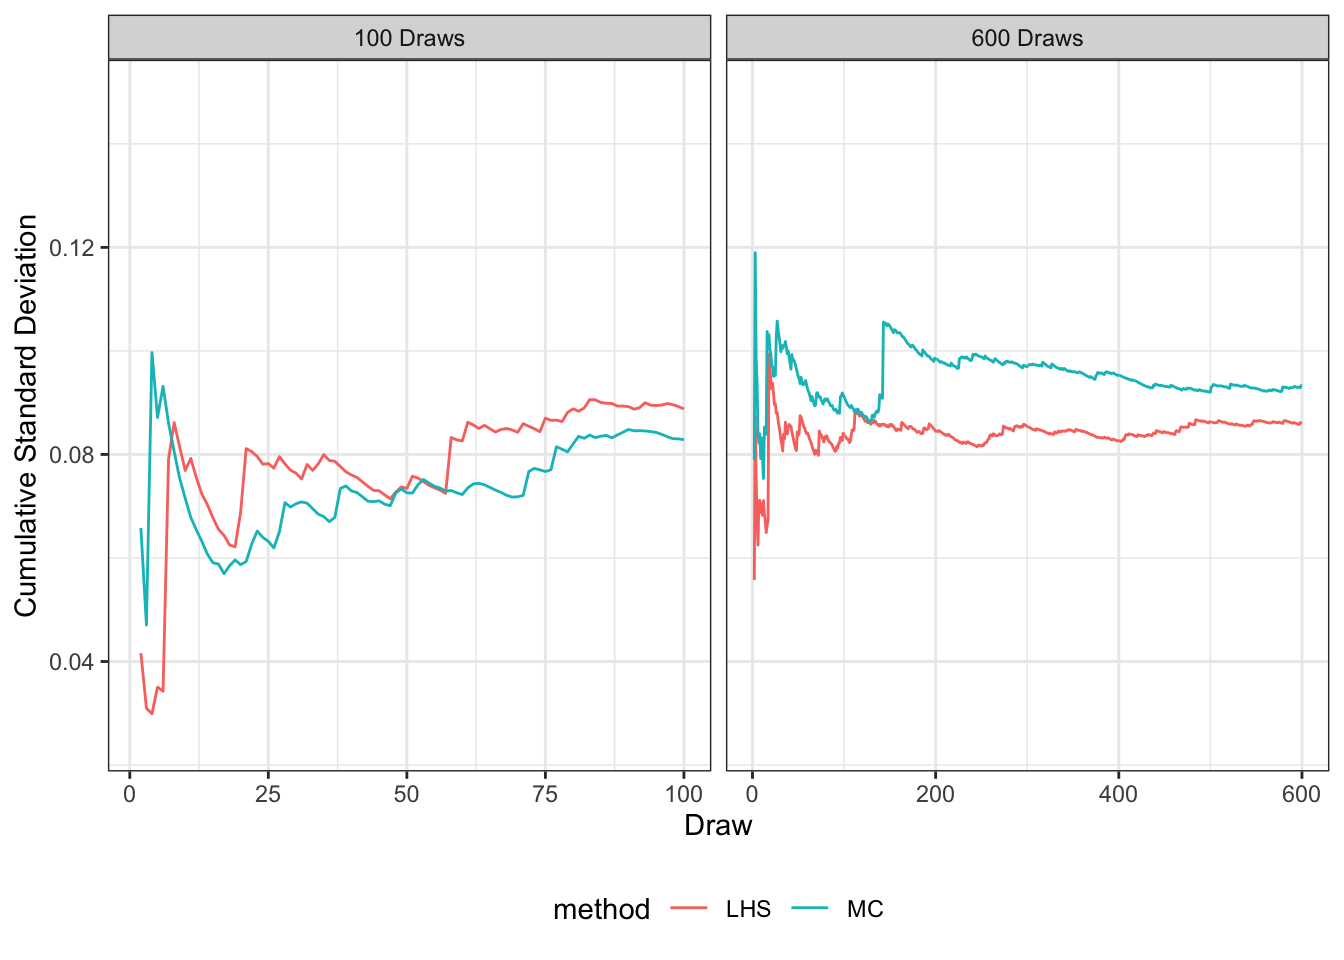
\includegraphics[width=0.75\linewidth]{ustm_resiliency_sensitivity_files/figure-latex/hbostats-1} 

}

\caption{HBO Mean Logsum Standard Variation with 100 and 600 Draws}\label{fig:hbostats}
\end{figure}

\begin{figure}

{\centering 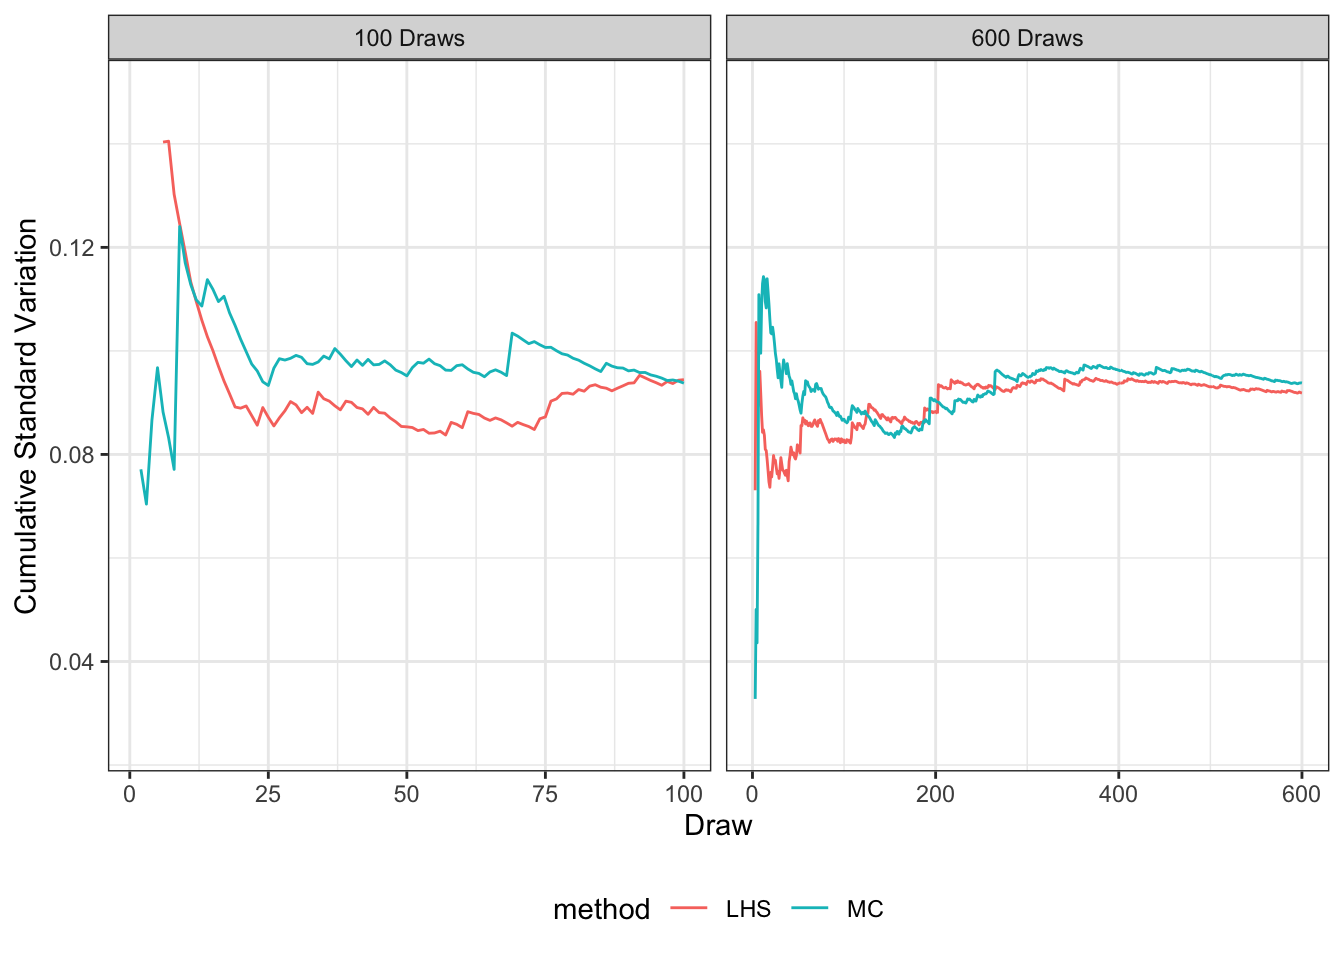
\includegraphics[width=0.75\linewidth]{ustm_resiliency_sensitivity_files/figure-latex/nhbstats-1} 

}

\caption{NHB Mean Logsum Standard Variation with 100 and 600 Draws}\label{fig:nhbstats}
\end{figure}

For all three trip purposes, the LHS method had its standard deviation stabilized between 100 and 200 draws. The MC method had still not stabilized to the same extent after 600 draws. This shows us that Latin Hypercube Sampling greatly decreases the iterations needed to approximate random sampling methods. Since LHS captures the possible variance at a small enough amount of iterations, it can and will be used for a statewide model.

\bibliography{book.bib}


\end{document}
